\documentclass[12pt]{article}

\usepackage{amsmath,amsthm,amssymb,amsfonts}
\usepackage[margin=1in]{geometry} 
\usepackage{graphicx}
\usepackage[all]{xy}
\usepackage{ dsfont }
\usepackage{float}
\usepackage{tikz}
\usepackage{subcaption}
\usepackage{xcolor}
\usetikzlibrary{knots}
\tikzset{knot/.style={double=#1,double distance=1pt,line width=2pt,white}}
\usepackage{amsmath,amsthm,amssymb,amsfonts}
 
\newcommand{\N}{\mathbb{N}}
\newcommand{\Z}{\mathbb{Z}}
 
\newtheorem{definition}{Definition}[section] 

\newenvironment{theorem}[2][Theorem]{\begin{trivlist}
\item[\hskip \labelsep {\bfseries #1}\hskip \labelsep {\bfseries #2.}]}{\end{trivlist}}
\newenvironment{lemma}[2][Lemma]{\begin{trivlist}
\item[\hskip \labelsep {\bfseries #1}\hskip \labelsep {\bfseries #2.}]}{\end{trivlist}}
\newenvironment{problem}[2][Problem]{\begin{trivlist}
\item[\hskip \labelsep {\bfseries #1}\hskip \labelsep {\bfseries #2.}]}{\end{trivlist}}

\newenvironment{example}[2][Example]{\begin{trivlist}
\item[\hskip \labelsep {\bfseries #1}\hskip \labelsep {\bfseries #2.}]}{\end{trivlist}}

 
\begin{document}
 
%\renewcommand{\qedsymbol}{\filledbox}
%Good resources for looking up how to do stuff:
%Binary operators: http://www.access2science.com/latex/Binary.html
%General help: http://en.wikibooks.org/wiki/LaTeX/Mathematics
%Or just google stuff
 
\title{Klein Links}
\author{Gary Guth, Yitz Deng, Kaavya Jayram}
\maketitle

\section{Basics of Klein Links}

A knot in mathematics is an embedding of a circle $S_1$ in $\mathbb{R}_3$. We can extend this definition of a knot to the idea of torus links. The $(m, n)$ torus link winds $m$ times around the meridian and $n$ times around the longitude. A known result is that the $(m,n)$ torus link has $\gcd(m,n)$ components.

\begin{figure}[H]
\centering
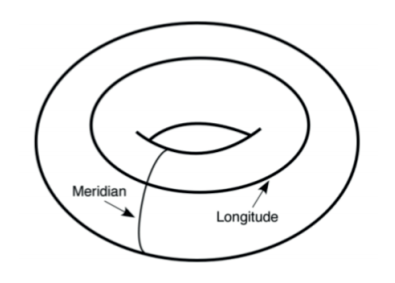
\includegraphics{meridianlongitude}
\caption{\label{Torus} Surface of a torus, showing the meridian and longitude. (\textit{Freund, Smith-Polderman})}
\end{figure}

If we cut a torus with a torus link on it along the longitude, we can mold the surface into a cylinder. We can then cut the cylinder along the longitude and deform it into a rectangle, with orientation:



\begin{figure}[H]
\centering
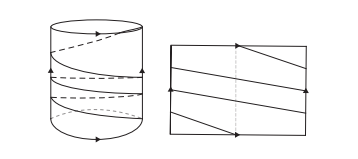
\includegraphics{deformtorusknot}
\caption{\label{Klein knot formation p1} Cutting and deforming a torus with a knot lying on the surface into a rectangle. (\textit{Freund, Smith-Polderman})}
\end{figure}


We can reverse the orientation of the bottom edge of the rectangle. Gluing back together the vertical sides creates a cylinder with edges in opposite orientations. To ensure that we connect this cylinder back to itself correctly, we must twist one side of the cylinder, and we do this by passing the cylinder through itself. 

\begin{figure}[H]
\centering
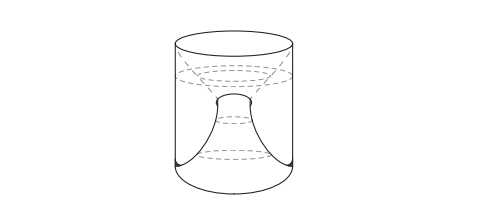
\includegraphics{kleinrep}
\caption{\label{Klein bottle representation} 3-dimensional representation of a Klein bottle. (\textit{Freund, Smith-Polderman})}
\end{figure}

This results in a hole, because of the intersection of the cylinder with itself. We place this hole in the upper left corner of the rectangle. 

\begin{figure}[H]
\centering
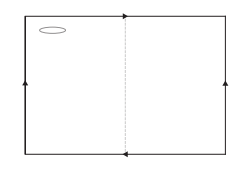
\includegraphics{kleinknot}
\caption{\label{Klein rectangle} The surface of a Klein bottle, represented as a rectangle. (\textit{Freund, Smith-Polderman})}
\end{figure}

For example, the $K(4, 3)$ is shown below on the rectangle. 

\begin{figure}[H]
\centering
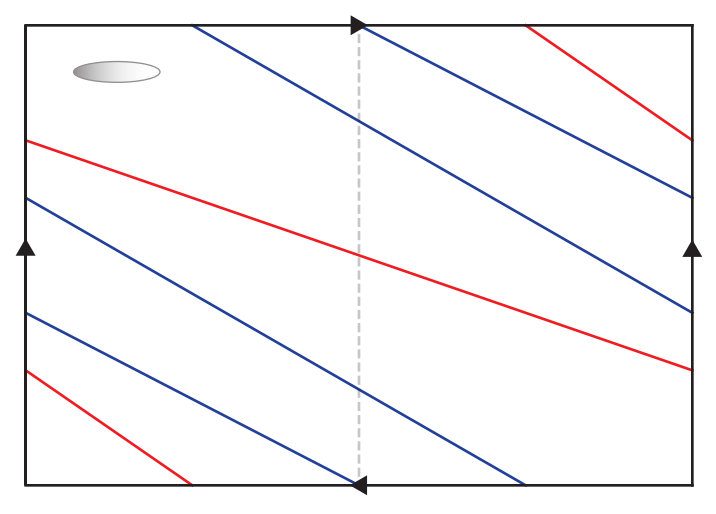
\includegraphics[width=3in]{k43}
\caption{\label{K(4, 3)} Example of the $K(4, 3)$ Klein link, represented on the rectangle. (\textit{Bowen})}
\end{figure}

We ensure that no strand on the rectangle is on the hole by ensuring that all strands connected to the top edge of the rectangle are above the hole, and all strands connected to the left edge of the rectangle are below the hole. 




We can now discuss the braid representation of a Klein link. It is a well-known fact that the braid representation of the $(m, n)$ torus knot is $(\sigma _1 ...\sigma _{n-1})^m$. In order to represent the $(m,n)$ Klein link, we compose the representation for the torus knot with a $180^{\circ}$ half-twist to the left as we look down on the cylinder. This results in $(\sigma _1 ...\sigma _{n-1})^m\prod_{i=1} ^{n-1} (\sigma_{n-1}^{-1}...\sigma_{i}^{-1})$.

\begin{figure}[H]
\centering
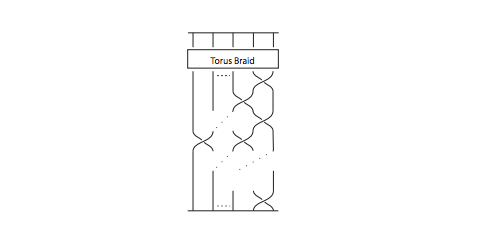
\includegraphics{braidrepklein}
\caption{\label{Braid rep klein knot} The twist that forms the braid representation of the Klein link. (\textit{Freund, Smith-Polderman})}
\end{figure}

Given this braid representation of a Klein knot, a connection between $K(m, 2)$ and $T(m-1, 2)$ becomes clear.  

\begin{theorem}{1.1} (\textit{Freund, Smith-Polderman})
The $K(m, 2)$ Klein link is isotopic to the $T(m-1, 2)$ torus link. 
\end{theorem}

\begin{proof}
This proof is straightforward by examining their braid representations. 

The $K(m, 2)$ Klein link can be represented as $(\sigma_1)^m (\sigma_1^{-1}) = \sigma_1^{m-1}$, while the $T(m-1, 2)$ torus link is represented as $\sigma_1^{m-1}$. They are equivalent. 
\end{proof}


Having reviewed some established properties of Klein Links, we now aim to extend the current understanding. We will now study the genus of Klein Links.

\section{Minimal Genus of a Klein Link}

To calculate the genus of our Klein Links, we will need the number of components in each link. It is a well known fact that the number of components in a $(m, n)$-torus link is the greatest common divisor of $m$ and $n$. So we must simply analyze what the half twist does to the number of components in the link.

\subsection{Components in a Klein Link}

A clever proof in Bowen's paper proves the following theorem. We will give a short overview of the proof.

\begin{theorem}{2.1} (\textit{Bowen13})
Let $m, n \in \mathds{N}$. If $m$ is even, then the $(m, n)$-Klein link has $\lceil \frac{n}{2} \rceil$  components. If $m$ is odd then the $(m, n)$-Klein link has $\lceil \frac{n + 1}{2} \rceil$ components. We will denote the number of components $C(m, n)$.
\end{theorem}

To prove this theorem, we will need to set up some machinery. 

First, note there is a natural homomorphism from the braid group on $n$-strands to the symmetry group on $n$ elements: $\pi:B_n \rightarrow S_n$, which maps $\sigma_i \mapsto (i \quad i+1)$. So we will define $T_n^m :=\pi(T(m, n)) = (1 \, n \, n-1 , ... , 2)^m$ and $K_n :=\pi(\Delta_n) = (1 \, n) (2 \, n-1) ... \left(\lceil\frac{n}{2}\rceil \, \lceil \frac{n+1}{2}\rceil \right)$.  Now that we have redefined our Torus and Klein braids as permutations, we can consider the group action of these permutations on the set $[n] := \{1, ..., n\}$.

\begin{definition}
Let $G$ be a group and $X$ a set. The \textbf{group action} $\phi$ of $G$ on $X$ is the map $$\phi:G\times X \rightarrow X : \, (g, x) \mapsto \phi(g, x)$$ satisfying $ex = x$ for all $x \in X$ and $(gg')x = g(g'x)$ for all $g, g' \in G$ and $x\in X$.

The \textbf{fix} of $g \in G$ is the set $fix(g) = \{x \in X: gx = x \}$. The \textbf{orbit} of $x$ in $X$ is the set $orb_G(x) = \{gx : g \in G \}$
\end{definition}

With these tools, we can reframe our problem of the number of components in the language of group actions. We will consider the group action of $\langle T_n^m K_n \rangle$ (the subgroup of $S_n$ generated by $T_n^m K_n$) on $[n]$. The number of orbit is exactly the number of components of the Klein Link. Using Burnside's Theorem, this quantity is easily calculated.

\begin{theorem}{2.2}
Given a group $G$ acting on a set $X$ the number of orbits $|X/G|$ is given by

\begin{equation}
|X/G| = \frac{1}{|G|}\sum_{g\in G} |fix(g)|
\end{equation}
\end{theorem}

To prove theorem 2.2 , we will need the order of $\langle T_n^m K_n \rangle$. It is easy to check that the order of $\langle T_n^m K_n \rangle$ is $2$ if $n>2$. With this we can compute the number of components in a Klein Link.

\begin{proof}
First, we consider the $n = 1$ case. Trivially $|fix(1)| = 1$, and $|\langle T_1^m K_1 \rangle| = 1$. So the number of orbits is $$\left|[1]/\langle T_1^m K_1 \rangle \right|= \frac{1}{1}(1) = 1$$ which is indeed $\lceil \frac{1 + 1}{2} \rceil$ and $\lceil \frac{1}{2}\rceil$. 

Now we consider $n = 2$. In this case, we have $|fix(1)| = 2$. If $m$ is odd $\langle T_2^m K_2 \rangle = (1)$, so $|\langle T_2^m K_2 \rangle| = 1$. Then $$|[2]/\langle T_2^m K_2 \rangle| = \frac{1}{1}(2) = 2 = \left\lceil \frac{2 + 1}{2}\right\rceil.$$ If $m$ is even, $\langle T_2^m K_2 \rangle = \{(1), (1 \, 2) \}$, so $|\langle T_2^m K_2 \rangle| = 2$. Then $$|[2]/\langle T_2^m K_2 \rangle| = \frac{1}{2}(2 + 0) = 1 = \left\lceil \frac{2}{2}\right\rceil.$$

Now we consider the case $n>2$. As stated before $|\langle T_n^m K_n \rangle| = 2$, and $fix(1) = n$. So all that remains is to calculate $|fix(T_n^m K_n)|$. We are looking for $i \in [n]$ such that $T_n^m K_n(i) = i$.

First, note that it follows from the permutation representations of $T_n^m$ and $K_n$ that $T_n^m(i) = i - m \quad \mod \, n$ and $K_n(i) = 1 - i \quad \mod \, n$. So we are looking to solutions to the modular equation $T_n^m K_n(i) = i$.

$$
T_n^m K_n(i) = T_n^m(1 - i) = 1 - i - m = 1 \quad \mod n
$$

So we need solutions to the equation:

\begin{equation}
2i = 1 - m \quad \mod n.
\end{equation}

If $n$ is odd, $\gcd(2, n) = 1$, so $2$ is a unit in $\mathds{Z}_n$, so the equation has a single solution, which then implies that $|fix(T_n^m K_n)|=1$. Therefore, 

$$
\left| [n]/\langle T_n^m K_n \rangle \right| = \frac{1}{2}(n + 1) = \left \lceil \frac{n + 1}{2} \right \rceil.
$$

If both $n$ and $m$ are even, the $\gcd(2, n) = 2$. Because $m$ is even, $1-m$ is odd, which means there are no solutions to the equation. Then we have 

$$
\left| [n]/\langle T_n^m K_n \rangle \right| = \frac{1}{2}(n + 0) = \left \lceil \frac{n}{2} \right \rceil.
$$

Finally, if $n$ is even and $m$ is odd, we still have $gcd(2, n) = 2$ and $1-m$ s even. Then we have $2$ solutions to the above equation, which implies $|fix(T_n^m K_n)| = 2$. So 

$$
\left| [n]/\langle T_n^m K_n \rangle \right| = \frac{1}{2}(n + 2) = \left \lceil \frac{n + 1}{2} \right \rceil.
$$
\end{proof}

\subsection{Minimal Genus}

\begin{definition}
A \textbf{positive braid} is a braid with only positive crossings.
\end{definition}

We state without proof the following theorem:

\begin{theorem}{2.3}
Seifert's algorithm produces a Seifert Surface with minimal genus for the closure of positive braids.
\end{theorem}

Recall we defined the braid representation of a Klein Link to be $K(m, n) = T(m, n) \Delta^{-1}_n$. We added a "negative" half twist in our definition of the Klein Link, which was convenient. This braid expression contains many negative crossings, so we cannot guarantee that Seifert's algorithm will produce a minimal genus surface. Fortunately, with a bit of manipulation, we can simplify our braid word and in doing so eliminate all minimal crossings.

\begin{theorem}{2.4}
For the $K(m, n)$ ($m \geq n$) a simplified braid word is:

\end{theorem}
\begin{equation}
K(m, n) = (\sigma_1 \sigma_2 ... \sigma_{n-1})^{m-n+1}(\sigma_1 \sigma_2...\sigma_{n-2})...\sigma_1
\end{equation}

\begin{proof}
\begin{align*}
K(m, n) &= (\sigma_1 \sigma_2 ... \sigma_{n-1})^m (\sigma_{n-1}^{-1} \sigma_{n-2}^{-1}... \sigma_1^{-1})...\sigma_1^{-1}\\
&=(\sigma_1 \sigma_2...\sigma_{n-1})^{m-1}(\sigma_{n-1}^{-1} \sigma_{n-2}^{-1}...\sigma_2^{-1})...\sigma_{n-1}^{-1} \\
&=(\sigma_1 \sigma_2...\sigma_{n-1})^{m-2}\sigma_1 (\sigma_{n-1}^{-1} \sigma_{n-2}^{-1}...\sigma_3^{-1})...\sigma_{n-1}^{-1}  \\
&= (\sigma_1 \sigma_2...\sigma_{n-1})^{m-2} (\sigma_{n-1}^{-1} \sigma_{n-2}^{-1}...\sigma_3^{-1})...\sigma_{n-1}^{-1} \sigma_1 \\
&=  \hspace{1in} \vdots \\
&= (\sigma_1 \sigma_2...\sigma_{n-1})^{m-n+1}(\sigma_1 \sigma_2 ... \sigma_{n-2})...\sigma_1 \\
\end{align*}
\end{proof}



So, now with this new positive braid representation we can now attack the problem of a minimal genus. 


\begin{theorem}{2.4}
The minimal genus $g_K$ of a positive Klein link $K^+(m, n)$ is 

\begin{equation}
g_K =  1 - \frac{1}{2}\left(n - (m - n + 1)(n-1) - \frac{(n-2)(n-1)}{2} + C(m, n)\right)
\end{equation}
\end{theorem}

\begin{proof}
To find the minimal genus, we will calculate the Euler Characteristic of the surface generated by Seifert's algorithm (which by theorem 2.3 has minimal genus). The Euler characteristic of a Seifert surface is the number of Seifert disks, minus the number of bands ($\chi = D - B$). So let's consider an $(m, n)$ - Klein Link (figure \ref{Klein link}).


\begin{figure}[H]
\centering
\begin{subfigure}{.7\textwidth}
  \centering
  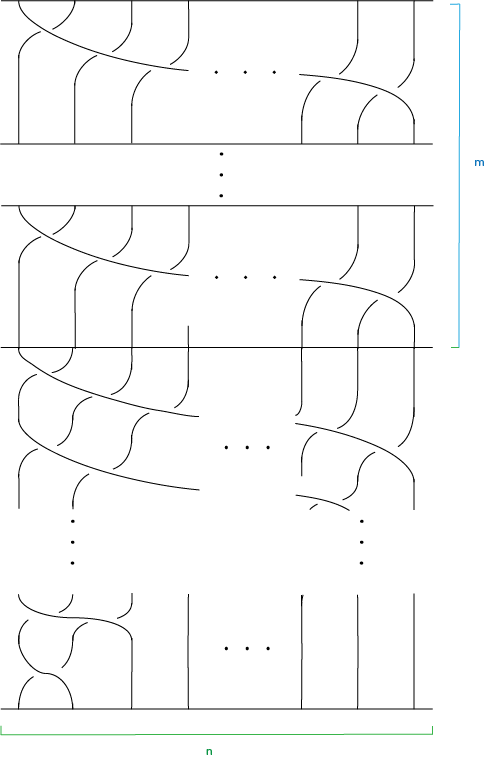
\includegraphics[width=.4\linewidth]{Klein_link}
  \label{fig:sub1}
\end{subfigure}%
\begin{subfigure}{.7\textwidth}
  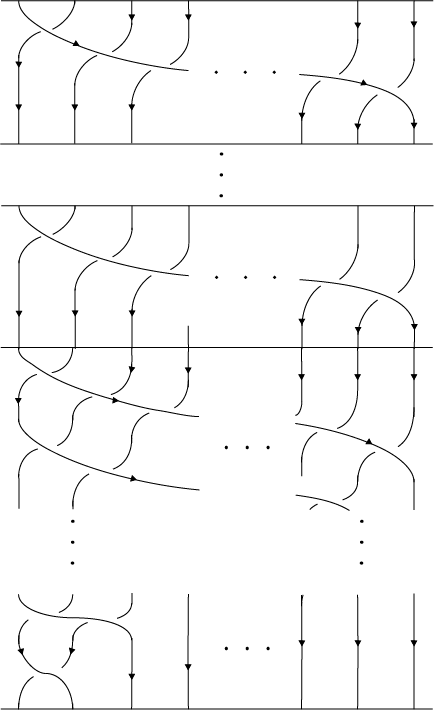
\includegraphics[width=.4\linewidth]{Klein_link_Oriented}
  \label{fig:sub2}
\end{subfigure}
\caption{\label{Klein link} An oriented $(m, n)$ - Klein link ($m$ full twists followed by a half twist on $n$ strings).}
\label{fig:test}
\end{figure}

To begin Seifert's algorithm, we must orient our knot. Fortunately, the braid representation makes it very clear how the Seifert disks are formed. In altering the crossings, every crossing is eliminated. So we are left with the closure of the identity braid, which means there is a single Seifert disk for each strand of the braid, or $D = n$.

\begin{figure}[H]
\centering
\begin{subfigure}{.7\textwidth}
  \centering
  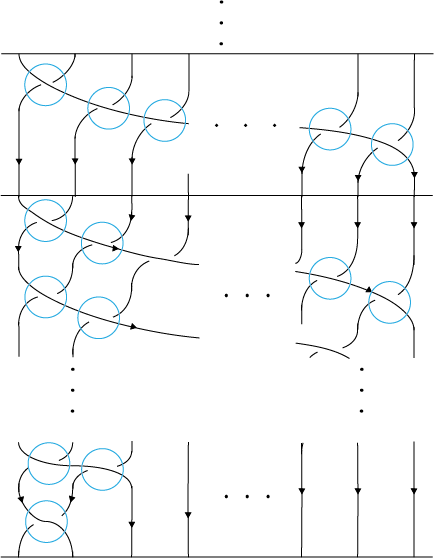
\includegraphics[width=.4\linewidth]{Klein_link_Seifert_Circles_Switch}
  \label{fig:sub1}
\end{subfigure}%
\begin{subfigure}{.7\textwidth}
  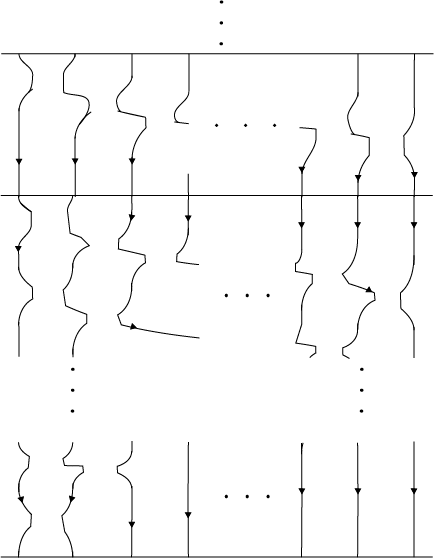
\includegraphics[width=.4\linewidth]{Klein_link_Seifert_Disks}
  \label{fig:sub2}
\end{subfigure}
\caption{\label{Crossing Switch} Removing crossings to make Seifert disks.}
\label{fig:test}
\end{figure}

So we now must simply count the number of bands. The number of bands is the number of crossings, or equivalently the number of $\sigma_i$ in the braid word.  Recall the braid word for a $(m, n)$ - Klein link is:

$$
K(m, n) = (\sigma_1 \sigma_2... \sigma_{n-1})^{m-n+1}(\sigma_1 \sigma_2... \sigma_{n-2})(\sigma_1 \sigma_2... \sigma_{n-3})...\sigma_1
$$

So the number of elements in the braid word is:

$$
B = (m - n + 1)(n - 1) + \sum_{k = 1}^{n-2}k = 
$$

\begin{equation}
B = (m - n + 1)(n - 1) + \frac{(n-2)(n-1)}{2}
\end{equation}

With this, we can now conclude the genus of $K(m, n)$.

$$
\chi = D - B = n - (m - n + 1)(n-1) - \frac{(n-2)(n-1)}{2} = 2 - 2g_k - C(m, n)
$$

Rearranging:

$$
g_K = 1 - \frac{1}{2}\left(n - (m - n + 1)(n-1) - \frac{(n-2)(n-1)}{2} + C(m, n)\right).
$$

\end{proof}

\section{Jones' Polynomial}

In this section, we will discuss finding the Jones polynomial for Klein Links. We explored a few different approaches. We first investigated imitating Jones' derivation for the polynomial for a torus knot, and then explored some algorithmic approaches to calculating Jones polynomials for the Klein links. 

\begin{definition} {(Jones)}

The \textbf{Jones polynomial} of a link $L$, $V(L)$, is a knot-invariant polynomial defined by the following properties: 

\begin{itemize}
\item Two isotopic knots have the same Jones polynomial.

\item The Jones polynomial of the unknot is 1. 

\item For a link $L$, there exists the skein relation $$t^{-1} V(L_+) - t V(L_-) = (t^{1/2} - t^{-1/2}) V(L_0)$$ where $L_+$, $L_-$, and $L_0$ are three oriented diagrams of the link $L$, with the sole difference being at one crossing of $L$ where $L_+$, $L_-$, and $L_0$ replace the original crossing with the corresponding crossing drawn below. 

\begin{figure}[H]
\centering
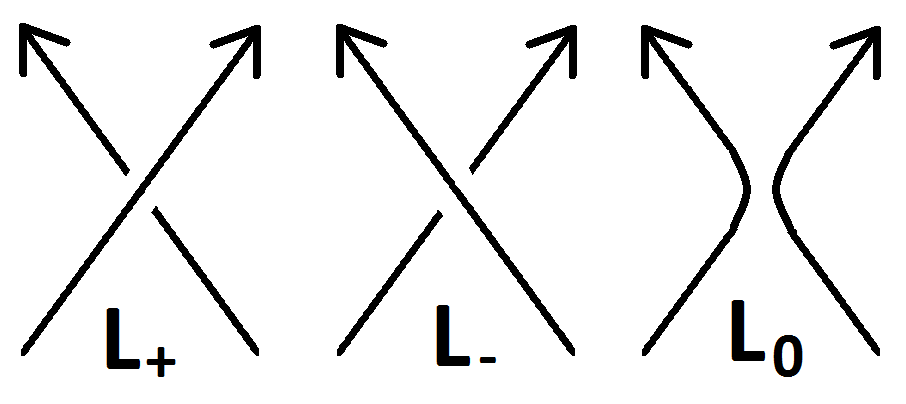
\includegraphics[width=3.5in]{threeLs}
\caption{\label{Jones Crossings} $L_+$, $L_-$, and $L_0$ replace a crossing on an oriented diagram of $L$ with the respective crossing shown above}
\end{figure}

\end{itemize}

\end{definition}

\subsection{Bracket Polynomial} 

Our first method of approach was to use the \textbf{bracket polynomial}, by representing Klein links into the Temperley-Leib Algebra. 

\begin{definition} {(Kauffman)}
A \textbf{bracket polynomial} of a link $L$ is a polynomial in the variable $A$n, restricted by the following three properties: 
\begin{itemize}
\item The bracket polynomial of the unknot is 1. 

\item \(\langle \tikz[baseline=-.8ex] \node[knot under cross,knot,draw,double=red] {}; \rangle = A \langle \tikz[baseline=-.8ex] \node[knot vert,knot,draw,double=red] {}; \rangle + A^{-1} \langle \tikz[baseline=-.8ex] \node[knot horiz,knot,draw,double=red] {}; \rangle\)

\item The bracket polynomial of the disjoint union of an unknot and a knot $L$ is equal to $-A^2 - A^{-2}$ times the bracket polynomial of $L$. 

\end{itemize}
\end{definition}

The bracket polynomial for a link $L$ is denoted $\langle L \rangle$. 

A key issue, however, arises in that the bracket polynomial is not invariant under type-1 Reidemeister move. To solve this problem, we can use what is called a "normalized" bracket polynomial. 

\begin{definition}
The \textbf{writhe} of a knot is calculated by assigning $1$ to all positive crossings, $-1$ to all negative crossings, and adding together all of these values. 
\end{definition}

\begin{definition} {(Kauffman)}
The \textbf{normalized bracket polynomial} (also known as the \textbf{Kauffman $X$-polynomial} of a knot $K$, $\langle \bar{K} \rangle$, is the polynomial obtained from multiplying $\langle K \rangle$ by $(-A^3)^{-W}$, where $w$ is the writhe of the knot. 
\end{definition}
\begin{theorem}{3.1}
The normalized bracket polynomial of a knot $K$ is knot-invariant. 
\end{theorem}
\begin{proof}

To show that the normalized bracket polynomial is knot-invariant, we show that across all three types of Reidemeister moves, the polynomial does not change. 

\begin{itemize}

\item We begin with the first Reidemeister move. Suppose that we have knot $K$, and $K'$ is the same knot $K$, except for one extra Type-1 Reidemeister move added in some place. This changes a straight line into a loop with a crossing. First, let us assume that this crossing is positive. 

Let the original knot $K$ have bracket polynomial $\langle K \rangle$ and writhe $w$. Then, the original knot $K$ has normalized bracket polynomial $\langle \bar{K} \rangle = (-A^3)^{-w} \langle K \rangle$. 

The new knot $K'$ has writhe $w + 1$, as we insert one positive crossing.  By the second property of a bracket polynomial, we can see that $$\langle K' \rangle = A (-A^2 - A^{-2}) \langle K \rangle + A^{-1} \langle K \rangle = -A^{3} \langle K \rangle.$$

Thus, the normalized bracket polynomial of $K'$ is $$\langle \bar{K'} \rangle = (-A^3)^{-(w + 1)} -A^3 \langle K \rangle = (-A^3)^{-(w + 1) + 1} \langle K \rangle = (-A^3)^{-w} \langle K \rangle.$$

A similar proof shows that if $K'$ is derived from $K$ but with a single loop from a negative crossing, their normalized bracket polynomials are equal. 

Thus, over the Type-1 Reidemeister move, the normalized bracket polynomial is invariant. 

\item We can combine the cases for the Type-2 and Type-3 Reidemeister moves. As both the writhe and the bracket polynomial are invariant over Type-2 and Type-3 Reidemeister moves, if we derive $K'$ from a knot $K$ (both with writhe $w$) by performing either a Type-2 or a Type-3 move, $\langle \bar{K'} \rangle = (-A^3)^{-w} \langle K' \rangle = (-A^3)^{-w} \langle K \rangle = \langle \bar{K} \rangle.$

Thus, over both the Type-2 and Type-3 Reidemeister moves, the normalized bracket polynomial is invariant. 


\end{itemize}

Because the polynomial is invariant across all three Reidemeister moves, the normalized bracket polynomial must be knot-invariant. 

\end{proof}

From the bracket polynomial, we must find a connection to the Jones polynomial. This is easily done by comparing the skein relations of the Jones polynomial and the bracket polynomial. 

\begin{theorem}{3.2}{\textit{(Kauffman)}} 

The Jones polynomial can be found by calculating the normalized bracket polynomial, then substituting $A = t^{-1/4}$. 

\end{theorem}
\begin{proof}

The skein relation of the regular bracket polynomial is $$\langle \tikz[baseline=-.8ex] \node[knot under cross,knot,draw,double=red] {}; \rangle = A \langle \tikz[baseline=-.8ex] \node[knot vert,knot,draw,double=red] {}; \rangle + A^{-1} \langle \tikz[baseline=-.8ex] \node[knot horiz,knot,draw,double=red] {}; \rangle.$$

Similarly, we can conclude that $$\langle \tikz[baseline=-.8ex] \node[knot over cross,knot,draw,double=red] {}; \rangle = A \langle \tikz[baseline=-.8ex] \node[knot horiz,knot,draw,double=red] {}; \rangle + A^{-1} \langle \tikz[baseline=-.8ex] \node[knot vert,knot,draw,double=red] {}; \rangle $$

If we multiply the first line by $A$ and the second line by $A^{-1}$, then subtract the second from the first, we get $$A \langle \tikz[baseline=-.8ex] \node[knot under cross,knot,draw,double=red] {}; \rangle - A^{-1} \langle \tikz[baseline=-.8ex] \node[knot over cross,knot,draw,double=red] {}; \rangle = \langle \tikz[baseline=-.8ex] \node[knot horiz,knot,draw,double=red] {}; \rangle - \langle \tikz[baseline=-.8ex] \node[knot horiz,knot,draw,double=red] {}; \rangle + A^{2} \langle \tikz[baseline=-.8ex] \node[knot vert,knot,draw,double=red] {}; \rangle - A^{-2} \langle \tikz[baseline=-.8ex] \node[knot vert,knot,draw,double=red] {}; \rangle $$

which simplifies to 

$$A \langle \tikz[baseline=-.8ex] \node[knot under cross,knot,draw,double=red] {}; \rangle - A^{-1} \langle \tikz[baseline=-.8ex] \node[knot over cross,knot,draw,double=red] {}; \rangle = (A^2 - A^{-2}) \langle \tikz[baseline=-.8ex] \node[knot vert,knot,draw,double=red] {}; \rangle $$

This is nearly the same as the skein relation for the Jones polynomial. Now, let us assume that we have an arbitrary link $L$ for which we are calculating the Jones polynomial; consider this skein relation acting on one of the crossings of $L$, and orient the link $L$ such that each of the skein relation diagrams flows from bottom to top. 

Let the resolved crossing $L_0$ replace the crossing of $L$ (or, if there is naturally no crossing there, do nothing); and let the writhe of the resulting link be $w$. Then, applying the multiplication of $(-A^3)^{-w}$ for the appropriate writhe value, 

\begin{align*}
(-A^3)^{w + 1} A \langle \tikz[baseline=-.8ex] \node[knot under cross,knot,draw,double=red] {}; \rangle - (-A^3)^{w - 1} A^{-1} \langle \tikz[baseline=-.8ex] \node[knot over cross,knot,draw,double=red] {}; \rangle &= (-A^3)^w (A^2 - A^{-2}) \langle \tikz[baseline=-.8ex] \node[knot vert,knot,draw,double=red] {}; \rangle \\
(-A^3)^{1} A \langle \tikz[baseline=-.8ex] \node[knot under cross,knot,draw,double=red] {}; \rangle - (-A^3)^{-1} A^{-1} \langle \tikz[baseline=-.8ex] \node[knot over cross,knot,draw,double=red] {}; \rangle &= (-A^3)^0 (A^2 - A^{-2}) \langle \tikz[baseline=-.8ex] \node[knot vert,knot,draw,double=red] {}; \rangle \\
-A^4 \langle \tikz[baseline=-.8ex] \node[knot under cross,knot,draw,double=red] {}; \rangle + A^{-4} \langle \tikz[baseline=-.8ex] \node[knot over cross,knot,draw,double=red] {}; \rangle &= (A^2 - A^{-2}) \langle \tikz[baseline=-.8ex] \node[knot vert,knot,draw,double=red] {}; \rangle \\
A^4 \langle \tikz[baseline=-.8ex] \node[knot under cross,knot,draw,double=red] {}; \rangle - A^{-4} \langle \tikz[baseline=-.8ex] \node[knot over cross,knot,draw,double=red] {}; \rangle &= (A^{-2} - A^{2}) \langle \tikz[baseline=-.8ex] \node[knot vert,knot,draw,double=red] {}; \rangle \\
\end{align*}

From this point, it is obvious that if we let $A = t^{-1/4}$, then we have exactly the skein relation of the Jones polynomial. Thus, finding the normalized bracket polynomial then letting $A = t^{-1/4}$ gives us the Jones polynomial, as all of its properties are met. 

\end{proof}

\subsubsection{Temperley-Leib Algebra}

\begin{definition}
An \textbf{algebra} over a commutative ring $R$ is an abelian group $A$, which has the structure of both a ring and an $R$-module which satisfies, for all $r \in R$ and $a, b \in A$, 

$$
r (xy) = (rx)y = x(ry)
$$.
\end{definition}



\begin{definition}
Let $R$ be the ring $\Z[A, A^{-1}]$, the ring of all polynomials in terms $A$ and $A^{-1}$ with integer coefficients. Let us fix $\tau \in R$. The \textbf{Temperley-Lieb Algebra} $TL_n(\tau)$ is the $R$-algebra generated by $n-1$ generators $\{e_1, ..., e_{n-1}\}$, subject to the following properties:

\begin{itemize}
\item $e_i^2 = \tau e_i$
\item $e_i e_j = e_j e_i \quad |i - j| > 1$
\item $e_i e_{i \pm 1} e_i = e_i$
\end{itemize}

A \textbf{tangle} is an element of a $TL_n(\tau)$ algebra. 
\end{definition}

The $i$th generator of a $TL_n$ algebra connects the top row to the bottom row as an identity mapping, except for the $i$th and $(i+1)$th nodes. Instead, the top two $i$th and $(i+1)$th node are connected, and the bottom two $i$th and $(i+1)$th node are connected. The generators for a $TL_n$ algebra can be diagrammatically shown below. 

\begin{figure}[H]
\centering
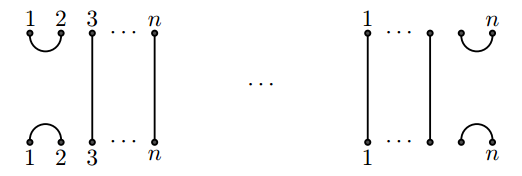
\includegraphics[width=4in]{tlgenerators}
\caption{\label{Temperley Leib} The element on the left is $e_1$ and the element on the far right is $e_{n-1}$.  (\textit{Abramsky})}
\end{figure}

These generators can be multiplied via the operation of concatenation. More specifically, when considering $\sigma_i \sigma_j$, we take the bottom row of $\sigma_i$ and the top row of $\sigma_j$ and connect them. Both rows have nodes numbered 1 to $n$; we connect the rows respectively. 
 
To connect $TL_n$ with our braids, we must correctly pick $\tau$ such that the union of an unconnected unknot with the rest of a tangle will be equivalent to left-multiplying the tangle by $\tau$, a valid operation of a module. Thus, we let $\tau = -A^2 - A^{-2}$, in order to agree with the properties of a bracket polynomial. . 
 
With these generators explicitly described, the three properties described above can be shown to be true. These properties are shown on a $TL_n$ tangle for small $n$, but it is clear that these properties will hold even when $n$ is increased.  First, we have $e_i^2 = \tau e_i$: 

\begin{figure}[H]

\centering
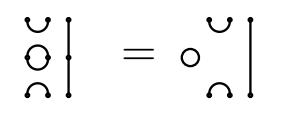
\includegraphics[width=3in]{tlproperty1}
\caption{\label{Prop 1} $e_i^2 = \tau e_i$. (\textit{Abramsky})}
\end{figure}

Next, we have $e_i e_{i \pm 1} e_i =e_i$. Only $e_i e_{i + 1} e_i = e_i$ is shown here; the reader can imagine, however, how the $e_i e_{i - 1} e_i = e_i$ property is true, just by flipping this diagram. 

\begin{figure}[H]

\centering
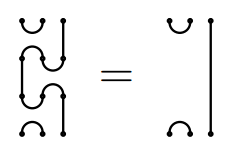
\includegraphics[width=3in]{tlproperty2}
\caption{\label{Prop 1} $e_i e_{i +1} e_i = e_i$. (\textit{Abramsky})}
\end{figure}




Lastly, we have $e_i e_j = e_j e_i$ when $|i - j| > 1$. This diagram specifically shows this property for $|i - j| = 2$, but by including straight strands in between $e_i$ and $e_j$, it is clear that this property holds for all $|i - j| > 1$. 
\begin{figure}[H]

\centering
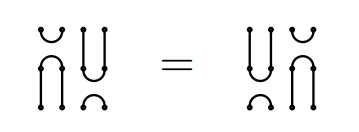
\includegraphics[width=4in]{tlproperty3}
\caption{\label{Prop 1} $e_i e_j = e_j e_i$ for $|i - j > 1$. (\textit{Abramsky})}
\end{figure}


As the identity of $TL_n(\tau)$ is just the tangle with no generators, it is equivalent to an $n$-unlink, and thus is equal to the identity of the braid group. We name this identity $1_n$. 

Now that we have defined Temperley-Leib Algebra and seen some of its properties, we can represent $n$-strand braids (and, specifically, the braid representation of a Klein knot) in $TL_n$. 

\begin{definition}
A \textbf{representation} of a group $G$ to an $R$ - algebra $A$ is a homomorphism $\rho: G \rightarrow A$.
\end{definition}

In our case, we wish to represent the braid group $B_n$ in $TL_n$. We thus define a homomorphism $\rho_n: B_n \rightarrow TL_n$, where $\rho_n(\sigma_i) = A 1_n+ A^{-1} e_i$ and $\rho_n(\sigma_i^{-1}) = A^{-1} 1_n + Ae_i$. Note that behavior of the identity is as expected; $1_n^j = 1_n$ for any $j \geq 1$, and $1_n e_i = e_i 1_n = e_i$ for any generator $e_i$. Most of the time, we will omit the $1_n$ when writing our representation; it is understood that any term without a generator is simply the $1_n$ term. 

To show that this homomorphism is a representation of the braid group $B_n$, we must show that the properties of the braid group are preserved; that is, the following relations are preserved through the homomorphism: 

$$\begin{cases}
\sigma_i \sigma_{i}^{-1} = 1 & i = 1  \dots, n - 1 \\
\sigma_i \sigma_{i + 1} \sigma_i = \sigma_{i + 1} \sigma_i \sigma_{i + 1} & i = 1, \dots, n - 2 \\
\sigma_i \sigma_j = \sigma_j \sigma_i & |i - j| > 1
\end{cases}$$

We tackle these cases one at a time. 

\begin{itemize} 
\item First, we show that the property that $\sigma_i \sigma_{i}^{-1} = 1$ is held through the homomorphism. We have
\begin{align*}
   \rho_n (\sigma_i \sigma_i^{-1}) &= \rho_n(\sigma_i) \rho_n(\sigma_i^{-1}) \\
   &= (A + A^{-1} e_i) (A^{-1} + A e_i) \\
   &= 1_n + A^2 e_i + A^{-2} e_i + e_i^2 \\
   &= 1_n + (A^2 + A^{-2}) e_i + \tau e_i \\
   &= 1_n + e_i [(A^2 + A^{-2}) + (-A^2 - A^{-2})] \\
   &= 1_n + e_i \cdot 0 \\
   &= 1_n
   \end{align*}
   
We can see that this first property holds true. 

\item Next, we show that $\sigma_i \sigma_{i + 1} \sigma_i = \sigma_{i + 1} \sigma_i \sigma_{i + 1}$. 
\begin{align*}
\rho_n(\sigma_i \sigma_{i + 1} \sigma_i) &= \rho_n (\sigma_i) \rho_n (\sigma_{i + 1}) \rho_n (\sigma_i) \\
&= (A + A^{-1} e_i) (A + A^{-1} e_{i + 1})(A + A^{-1} e_i) \\
&= A^3 + A e_i + A e_{i + 1} + A^{-1} e_{i + 1} e_i + A e_i + A^{-1} e_i^2 + A^{-1} e_i e_{i + 1} + A^{-3} e_i e_{i + 1} e_i \\
&= A^3 + A e_i + A e_{i + 1} + A^{-1} e_{i + 1} e_i + A e_i + A^{-1} \tau e_i + A^{-1} e_i e_{i + 1} + A^{-3} e_i \\
&= A^3 + (A + A + A^{-1} \tau + A^{-3}) e_i + A e_{i + 1} + A^{-1} e_{i + 1} e_i + A^{-1} e_i e_{i + 1} \\
&= A^3 + [2A + A^{-1} (-A^{2} - A^{-2}) + A^{-3}] e_i + A e_{i + 1} + A^{-1} (e_{i + 1} e_i + e_ie_{i + 1}) \\
&= A^3 + (2A - A - A^{-3} + A^{-3})e_i + A e_{i + 1} + A^{-1}(e_{i + 1} e_i + e_i e_{i + 1}) \\
&= A^3 + Ae_i + Ae_{i + 1} + A^{-1}(e_{i + 1} e_i + e_i e_{i + 1}) \\
&= A^3 + A(e_i + e_{i + 1}) + A^{-1}(e_{i + 1} e_i + e_i e_{i + 1}) \\
\end{align*}
\begin{align*}
\rho_n(\sigma_{i + 1} \sigma_{i} \sigma_{i + 1}) &= \rho_n (\sigma_{i + 1}) \rho_n (\sigma_i) \rho_n (\sigma_{i + 1}) \\
&= (A + A^{-1} e_{i + 1}) (A + A^{-1} e_{i})(A + A^{-1} e_{i + 1}) \\
&= A^3 + A e_{i + 1} + A e_{i} + A^{-1} e_{i} e_{i + 1} + A e_{i+1} + A^{-1} e_{i+1}^2 + A^{-1} e_{i+1} e_{i} + A^{-3} e_{i+1} e_{i} e_{i+1} \\
&= A^3 + A e_{i + 1} + A e_{i} + A^{-1} e_{i} e_{i + 1} + A e_{i+1} + A^{-1} \tau e_{i+1} + A^{-1} e_{i+1} e_{i} + A^{-3} e_{i+1} \\
&= A^3 + (A + A + A^{-1} \tau + A^{-3}) e_{i + 1} + A e_{i} + A^{-1} e_{i} e_{i+1} + A^{-1} e_{i+1} e_{i} \\
&= A^3 + [2A + A^{-1} (-A^{2} - A^{-2}) + A^{-3}] e_{i+1} + A e_{i} + A^{-1} (e_{i} e_{i+1} + e_{i+1} e_{i}) \\
&= A^3 + (2A - A - A^{-3} + A^{-3})e_{i+1} + A e_{i} + A^{-1} (e_{i} e_{i+1} + e_{i+1} e_{i}) \\
&= A^3 + Ae_{i + 1} + Ae_{i} + A^{-1} (e_{i} e_{i+1} + e_{i+1} e_{i}) \\
&= A^3 + A(e_{i+1} + e_{i}) + A^{-1} (e_{i} e_{i+1} + e_{i+1} e_{i}) \\
&= A^3 + A(e_i + e_{i + 1}) + A^{-1}(e_{i + 1} e_i + e_i e_{i + 1}) \\
   \end{align*}
   
   Again, we can see that this second property holds true. 
   
   \item Lastly, we show that for $| i - j| > 1$, $\sigma_i \sigma_j = \sigma_j \sigma_i$. 
   
   \begin{align*}
   \rho_n(\sigma_i \sigma_j) &= \rho_n(\sigma_i) \rho_n(\sigma_j) \\
   &= (A + A^{-1} e_i)(A + A^{-1} e_j) \\
   &= A^2 + e_j + e_i + A^{-2} e_i e_j \\ \\
   \rho_n(\sigma_j \sigma_i) &= \rho_n (\sigma_j) \rho_n (\sigma_i) \\
   &= (A + A^{-1} e_j)(A + A^{-1} e_i) \\
   &= A^2 + e_j + e_i + A^{-2} e_j e_i \\
   &= A^2 + e_i + e_j + A^{-2} e_i e_j 
   \end{align*}
   
   We can see that this third property holds true. Note that $e_j e_i = e_i e_j$ as this is true for $TL_n(\tau)$ when $|i - j| > 1$, which is part of our initial assumptions. 
   
   \end{itemize}
   
   Before we may begin analyzing the bracket polynomial, we must define two more terms. 
   
   \begin{definition}
   Let $E$ be some product (concatenation) of generators of $TL_n$; let the tangle represented by this product of generators be $T_E$. The \textbf{closure} of $T_E$ occurs by connecting the $n$ top ends of the tangle with the $n$ bottom ends of the tangle correspondingly. We connect the top row of the first generator in $E$ with the bottom row of the last generator in $E$, in an operation similar to concatenation. 
   \end{definition}
   
   By taking the closure of a tangle, we get a disjoint union of some number of unknots. Note that there are no crossings in any of the generators, and the concatenation operation does not create any crossings; thus, in the tangle, there are no crossings. Similarly to concatenation, the closure of a tangle does not create any tangles, as it simply creates $n$ loops. It must then be the case that the closure of a tangle is the disjoint union of some number of unknots. 
   
   \begin{definition}
   If $T_E$ is a tangle, then the \textbf{trace} of $T_E$ is the operation $tr(T_E)$ that counts the number of unknots in the tangle of the closure of $T_E$. 
   \end{definition}

	It may be noted that through the three properties of $TL_n$, the trace of a tangle does not change; in other words, the trace is tangle-invariant. 
    
\subsubsection{Bracket Polynomial, Revisited}

We can now return to the bracket polynomial and evaluate the bracket polynomial of a tangle $T_E \in TL_n$. We must, however, note a few things. 

Because the writhe of a knot is the number of positive crossings minus the number of negative crossings, and each knot can be represented as a braid, the writhe of a braid is similarly defined. But since every crossing in a braid is purely identified by the braid generators, the writhe of a braid is just the sum of exponents of the braid generators. For example, the braid $\sigma_1 \sigma_2^{-2} \sigma_4$ has writhe 0. 

As the normalized bracket polynomial is knot-invariant, it must also be braid invariant, as each knot can be represented as a braid according to a theorem by Alexander. 

The bracket polynomial of a knot (or a braid) is calculated by taking each crossing, considering the different knots/links (and polynomials) obtained by resolving the crossing in two separate ways, then multiplying those polynomials by $A$ or $A^{-1}$ depending on the direction of the resolution. By doing so to a braid, after all crossings have been resolved, we get elements of $TL_n$. 

In fact, in performing the representation $\rho_n$ by mapping any $\sigma_i$ to $(A 1_n  + A^{-1}e_i)$ and any $\sigma_i^{-1}$ to $(A^{-1}1_n  + A e_i)$, we are resolving crossings in two directions, in the same fashion as the property of the bracket polynomial. 

Thus, for each concatenation of $TL_n$ generators in the representation $\rho_n$ of a braid $B$, we calculate the bracket polynomial of the closure of those generators, then multiply by the corresponding coefficients of powers of $A$ and $A^{-1}$. Because the closure of any tangle in $TL_n$ is simply a disjoint union of some number of unknots, it follows that any bracket polynomial of the closure of some number of generators of $TL_n$ must be a power of $\tau = (-A^{-2} - A^{2})$.


\begin{theorem}{3.3}
If $E$ is a product of some number of generators of $TL_n$, then bracket polynomial of $E$ is equal to $\tau^{tr(E) - 1}$. 

\end{theorem}

\begin{proof}
The bracket polynomial of the unknot is $1$, and the unknot has trace $1$ when represented in $TL_n$. This agrees with the formula of the bracket polynomial, $\tau^{tr(O) - 1} = \tau^{0} = 1$. 

Consider a tangle $T$ in $TL_n$ with $tr(T) \geq 1$. Let us assume that $\tau^{tr(T) - 1}$ correctly represents the bracket polynomial of $T$. Now consider $T' \in TL_n$, where $tr(T') = tr(T) + 1$. By the formula, the bracket polynomial of $T'$ is $\langle T' \rangle = \tau^{tr(T)}$. By the properties of a bracket polynomial, as $T'$ is just the disjoint union of $T$ with an unknot, Thus, the bracket polynomial of $T'$ is equal to $\langle T' \rangle = (-A^{-2} - A^2) \langle T \rangle = \tau \cdot \tau^{tr(T) - 1} = \tau^{tr(T)}$. 

The bracket polynomial derived from the formula is equal to the bracket polynomial derived from its properties; thus, by the method of induction, the bracket polynomial of a tangle $T \in TL_n$ for any $n$ is $\langle T \rangle = \tau^{tr(T) - 1}$. 


\end{proof}

After we obtain the bracket polynomial, we must multiply by $(-A^3)^{-w}$, where $w$ is the writhe of the braid. As explained earlier, this value is simply the sum of the exponents over all generators in the braid polynomial. 

We now have the normalized bracket polynomial $\langle \bar{K}(m, n) \rangle$ of a Klein knot; however, we must find the corresponding Jones polynomial. As shown earlier, we can simply let $A = t^{-1/4}$ to find the Jones polynomial. 

\begin{example}{3.1}
For an example, let us consider the Klein knot represented by $K(4, 2)$; we determined earlier that this knot is isotopic to the trefoil. The $K(4, 2)$ Klein knot has braid representation $$B_{4, 2} = (\sigma_1)^4 \sigma_1^{-1}) = \sigma_1^3.$$ The $TL_2$ representation of $B_{4, 2}$ is $$\rho_2(B_{4, 2}) = (A + A^{-1} e_1)^3 = A^3 + 3A e_1 + 3A^{-1} e_1^2 + A^{-3} e_1^3.$$

In $TL_2$, the identity element has trace $2$, $e_1$ has trace $1$, $e_1^2$ has trace $2$, and $e_1^3$ has trace $3$. These four can be checked by simply drawing each tangle, then counting the number of unknots. Thus, the bracket polynomial of the trefoil is $$\langle K(4, 2) \rangle = \tau A^3 + 3A + 3\tau A^{-1} + \tau^2 A^{-3} = -A^5 - A^{-3} + A^{-7}.$$

(The writhe of the $K(4, 2)$ Klein knot is $3$, since it's represented by $\sigma_1^3$. Thus, to obtain $\langle \bar{K}(4, 2) \rangle$, we must multiply $\langle K(4, 2) \rangle$ by $(-A^3)^{-3} = -A^{-9}$, so $$\langle \bar{K}(4, 2) \rangle = A^{-4} + A^{-12} - A^{-16}$$

Letting $A = t^{-1/4}$, we can see that the Jones polynomial of the $K(4, 2)$ knot is $$V(K(4, 2)) = t + t^3 - t^4.$$ This agrees exactly with the confirmed Jones polynomial for the trefoil. 

\end{example}

The largest drawback to this method of bracket polynomials and Temperley-Leib algebra is that for a given Klein knot $K$, if the braid representation of $K$ contains a product of $m$ braid generators, the polynomial $\langle K \rangle$ will have $2^m$ terms before simplification. Though this was not an issue for our small example of $K(4, 2)$, this can easily pose a problem for larger, more complex Klein links. 

Instead of having to calculate this by hand, we created a computer program to calculate this polynomial for us. It is composed of an object that represents $TL_n$ algebra, allowing one to input $n$ as an argument to the object initiation. Then, given the order of $TL_n$ generators, the object has a method to exactly determine the trace of the tangle. The program then uses these capabilities to determine the bracket (and subsequently, the Jones polynomial) of a given $K(m, n)$ Klein knot. 

The hardest part of writing this program was coming up with a way to represent a ring with a non-abelian multiplicative structure, as using sympy and other regular tools assumes that your polynomials are abelian. The PolyPart class solves this issue, along with a special multiplication function to ensure that the generators $e_i$ are kept in the correct order. 

\begin{figure}[H]
\centering
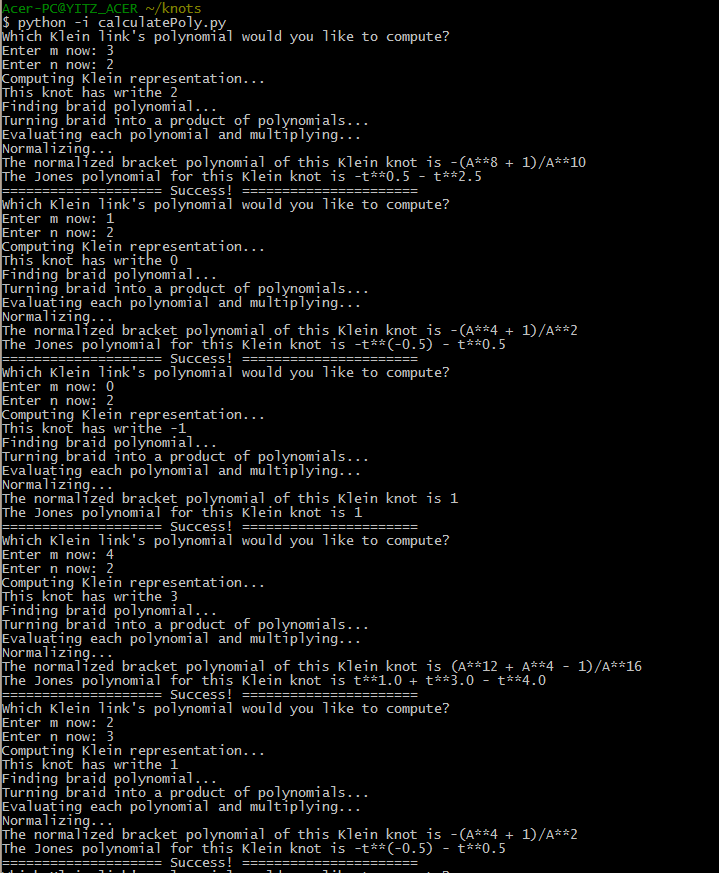
\includegraphics[width=6.5in]{kleincode}
\caption{\label{code} From top to bottom: $K(3, 2), K(1, 2), K(0, 2), K(4, 2), K(2, 3).$}
\end{figure}

Each of these Jones polynomials is correctly computed. The code is attached and clearly commented for the reader. 


\subsection{Skein Relations}

We also tried to directly use the skein relation for the Jones polynomial to calculate the Jones polynomial of a $K(m, n)$ Klein knot.

\begin{theorem}{3.4}

The Jones polynomial for the $K(0, 2)$ and $K(1, 2)$ Klein knots are $1$ and $-t^{1/2} - t^{-1/2}$, respectively. 

For a $K(m, 2)$ Klein knot with $m \geq 2$, the Jones polynomial can be calculated by the recursion  $$V(K(m, 2)) = t^2 V(K(m - 2, 2)) + (t \sqrt{t} - \sqrt{t}) V(K(m - 1, 2)).$$

\end{theorem}

\begin{proof}

As a $K(m, n)$ Klein knot can be represented by the braid representation $$K(m, n) = (\sigma_1 \dots \sigma_{n - 1})^m (\sigma_{n - 1}^{-1} \dots \sigma_1^{-1}) \dots \sigma_{n - 1}^{-1},$$

a $K(m, 2)$ knot can be simplified into the form $$K(m, 2) = \sigma_1^{m - 1}.$$

The $K(0, 2)$ Klein knot has braid representation $\sigma_1^{-1}$, and this is the unknot, so it has Jones polynomial 1. 

The $K(1, 2)$ Klein knot has braid representation $1$, and this is the 2-unlink. This is known to be $- t^{1/2} - t^{-1/2}.$ 

To apply the skein relation for $m \geq 2$, let us consider the last $\sigma_1$ crossing in the braid representation of $K(m, 2)$. $L_+$ would be the same as the original braid $\sigma_1^{m - 1}$, but $L_-$ would turn the last $\sigma_1$ into $\sigma_1^{-1}$, so the $L_-$ braid would actually be $\sigma_1^{m - 3} = K(m - 2, 2)$. Similarly, $L_0$ nullifies the last $\sigma_1$, so the $L_0$ braid is actually $\sigma_1^{m - 2} = K(m - 1, 2)$. 

The skein relation for the Jones polynomial can be rearranged to be $$V(L_+) = t^2 V(L_-) + (t \sqrt{t} - \sqrt{t}) V(L_0).$$ We can now replace $L_+$, $L_-$, and $L_0$ with their corresponding Klein knots to get $$V(K(m, 2)) = t^2 V(K(m - 2, 2)) + (t \sqrt{t} - \sqrt{t}) V(K(m - 1, 2)).$$

\end{proof}

\section{Conclusion}

Torus links are rather well documented in knot theory, and all kinds of properties have already been found. Through this paper, we have extend certain properties to Klein links, and we discover certain properties among Klein links. such as their genera, polynomials, and relations between Klein links and torus links. Along the way, we have created an algorithm that can calculate the Bracket and Jones polynomials for a Klein link, and, if parameters are changed, can work for any knot. 

\subsection{Open Questions}

As usual, we chanced upon certain questions to which we did not find answers, but left open-ended. 

\begin{itemize}

\item Is it possible to extend the Skein relation technique to find the Jones polynomial of a $K(m, 2)$ knot used in Theorem 3.4 to find the Jones polynomial of a general $K(m, n)$ knot? The polynomials for $K(m, 2)$ were easily found by simply realizing that $K(m, 2)$ can be simplified to $\sigma_1^{m - 1}$, while a simplification of $K(m, 3)$ into $(\sigma_1 \sigma_2)^{m - 2} \sigma_1$ seems many times more complex, and for larger $n$, the braid representation for $K(m, n)$ contains more and more terms. 

\item On the other hand, what is the closed form for Jones polynomials for $K(m, 2)$ links? Given its form as a "linear" recurrence relation (where functions themselves are treated as constants), it is likely that it has a closed form. We tried, however, to calculate the first few Jones polynomials for $K(m, 2)$ links for small $m$, and there appeared not to be an obvious pattern. 

\item What is the computational complexity of the algorithm provided? First, what is the complexity of the object and method to calculate trace, and what is the complexity of the function to calculate the polynomial itself? If the algorithm is rather inefficient, what can be done to improve its efficiency? 

\item It is hard to tell whether there are special cases in which the Jones polynomial is incorrect. By checking with an online catalog of Klein links (\textit{Bowen}) and knowing what the Jones polynomials are for simple links and knots, the Jones polynomials for small $m, n$ are confirmed to be correct through this algorithm. Originally, we had an issue with $K(m, 0)$ links, but this was resolved by noticing that any $K(m, 0)$ klein link is simply $m$ unknots and thus its bracket polynomial could be calculated by $\tau^{m - 1}$. 

\item Do there exist more connections between Klein links and torus links? It is possible that there is yet another connection left uncovered between Klein and torus links. 

\end{itemize}



\clearpage


\section{Bibliography}

\begin{itemize}

\item Fruend, David and Smith-Polderman, Sarah. \textit{Klein Links and Braids.} Rose-Hulman Undergraduate Mathematics Journal, Volume 14, No. 1, Spring 2013. \\ (https://www.rose-hulman.edu/mathjournal/archives/2013/vol14-n1/paper6/v14n1-6pd.pdf)

\item Abramsky, Samson. \textit{Temperley-Leib Algebra: From Knot Theory to Logic and Computation via Quantum Mechanics.} Mathematics of Quantum Computing and Technology, p415-458, 2007. \\ (http://www.cs.ox.ac.uk/samson.abramsky/tambook.pdf)

\item Kauffman, Louis. \textit{State Models and the Jones Polynomial.} Topology, Volume 26, No. 3, p395-407, 1987.  \\
(http://www.maths.ed.ac.uk/~aar/papers/kauffmanjones.pdf)

\item Jones, Vaughan. \textit{The Jones Polynomial.} \\ (https://math.berkeley.edu/~vfr/jones.pdf)

\item Bowen, Jennifer. \textit{Klein Link Catalogue.} \\ (http://discover.wooster.edu/jbowen/research/klein-links/digital-catalogue/)

\item Bowen, Jennifer et al. \textit{Klein Link Multiplicity and Recursion.} \\ (http://discover.wooster.edu/jbowen/files/2013/10/Klein-Link-Multiplicity-and-Recursion.pdf)


\end{itemize}

%%% Citations: 

% http://discover.wooster.edu/jbowen/research/klein-links/digital-catalogue/ as Bowen

% http://discover.wooster.edu/jbowen/files/2013/10/Klein-Link-Multiplicity-and-Recursion.pdf as Bowen13

\end{document}